\section{Analysis}
\subsection{Spectrophotometer Standardization}
\label{fig:spectrophotometer_standardization}
According to the Beer-Lambert Law described in \cref{eq:beer_lambert_law}, absorbance and concentration should follow a linear trend when \(0.05 < A < 1\). By creating solutions where \(Fe^{3+}\) is 100 times more abundant than \(SCN^-\), it is safe to assume that the \(SCN^-\) is entirely reacted to form the thiocyanatoiron complex (\cref{table:ice_standardization}). Thus, the precise linear trend between absorbance and concentration can be determined using these standard concentration samples. Sample calculations for the first standardization sample are shown below.

\begin{align}
    mol \; Fe^{3+} &= [Fe^{3+}]_{stock} \times V_{Fe^{3+}} = 1.00 \; M \times 2.00 \; mL \times \frac{1 \; L}{1000 \; mL} = 2.00 \times 10^{-4} \; mol \\
    mol \; SCN^- &= [SCN^-]_{stock} \times V_{SCN^-} = 0.001 \; M \times 5.00 \; mL \times \frac{1 \; L}{1000 \; mL} = 5.00 \times 10^{-6} \; mol \\
    [FeSCN^{2+}] &= \frac{mol \; SCN^-}{V_{total}} = \frac{2.00 \times 10^{-6} mol}{12 \; mL} \times \frac{1000 \; mL}{1 L} = 4.17 \times 10^{-4} \; M
\end{align}

\begin{table}[H]
\centering
\begin{tabular}{l|ll|l}
  & \(Fe^{3+}\) & \(SCN^-\) & \(FeSCN^{2+}\) \\ \hline
  
I & \(2.00 \times 10^{-4}\)                      & \(5.00 \times 10^{-6} \)
                      & 0                      \\ 
C & \(-5.00 \times 10^{-6} \)                     & \(-5.00 \times 10^{-6} \)                     & \(+5.00 \times 10^{-6}\)                      \\ 
E & \( 1.95 \times 10^{-4} \)                     & 0                      & \(5.00 \times 10^{-6} \)                \\ 
\end{tabular}
\caption{Moles ICE for First Spectrophotometer Standardization Sample}
\label{table:ice_standardization}
\end{table}

\noindent
\cref{eq:standardization_conc_uncertainty} is the formula to calculate the percent uncertainty of the standardization concentrations. The conversion factors and concentration of the solutions are assumed to have negligible uncertainty.

\begin{equation}
    \frac{\delta [FeSCN^{2+}]}{[FeSCN^{2+}]} = \frac{\delta V_{SCN^-}}{V_{SCN^-}} + \frac{\delta V_{total}}{V_{total}} = \frac{0.05 \; mL}{5.00 \; mL} + \frac{0.1 \; mL + 0.1 \; mL + 0.1 \; mL}{12 \; mL} = 2\% \label{eq:standardization_conc_uncertainty}
\end{equation}

\noindent
\cref{eq:standardization_absorbance} calculates the absorbance \(A\) from the transmittance \(T\). Note that absorbance has dimensionless Absorbance Units (AU). Sample calculations for the first standardization sample are shown below.

\begin{equation}
    A = \log_{10} \frac{1}{T} = \log_{10} \frac{1}{0.1559} = 0.8172 \; AU \label{eq:standardization_absorbance}
\end{equation}

\noindent
The uncertainty for \(A\) can be determined using the Law of Propagation of Uncertainty \citep{taylor_1982}.
\begin{equation}
    \delta f(x,y,\dots)=\sqrt{\left(\frac{\partial f}{\partial x}\delta x \right)^2+ \left(\frac{\partial f}{\partial y}\delta y \right)^2+\dots} \label{eq:general_uncertainty}   
\end{equation}

\noindent
Thus, for \(A=\log_{10} \frac{1}{T}\),
\begin{equation}
    \delta A = \delta \log_{10} \frac{1}{T} = \sqrt{\left(\frac{\partial \log_{10} \frac{1}{T}}{\partial T}\delta T \right)^2} = \frac{\delta T}{T \ln 10} = \frac{0.00035}{0.1559 \ln 10} = 0.0010 \; AU 
\end{equation}

\noindent
Repeating the above steps for each of the standardization samples results in \cref{table:absorbance_standard_concentrations} and \cref{fig:standardization_curve}.

\begin{table}[H]
\centering
\begin{tabular}{|C{2.5cm}|C{4cm}|C{2.5cm}|C{3.5cm}|}
\hline
Concentration (\(M\)) & Concentration Percent Uncertainty (\%) & Absorbance (\(AU\)) & Absorbance Uncertainty (\(AU\)) \\ \hline
\(4.17 \times 10^{-4}\)            & 2                                        & 0.8172             & 0.0010                          \\ \hline
\(3.33 \times 10^{-4}\)            & 3                                        & 0.7007             & 0.0008                          \\ \hline
\(2.50 \times 10^{-4}\)           & 3                                        & 0.5948             & 0.0006                          \\ \hline
\(1.67 \times 10^{-4}\)            & 4                                        & 0.4985             & 0.0005                          \\ \hline
\(8.33 \times 10^{-5}\)            & 6                                       & 0.3915             & 0.0004                          \\ \hline
\end{tabular}
\caption{Absorbance vs Standard Concentrations}
\label{table:absorbance_standard_concentrations}
\end{table}

\begin{figure}[H]
    \centering
    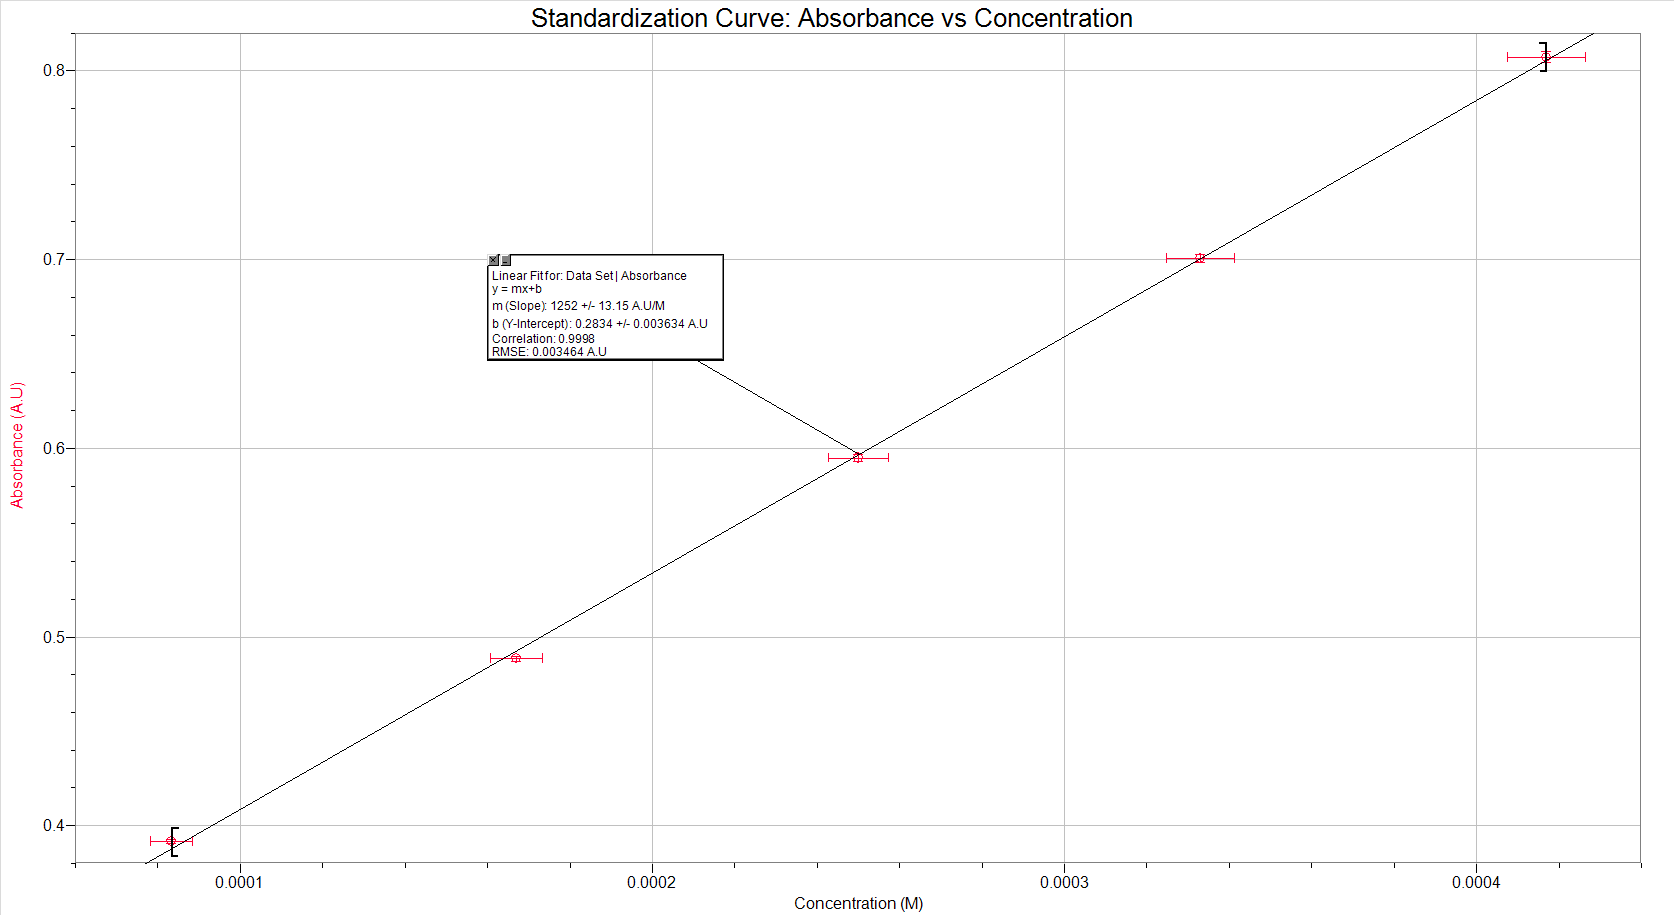
\includegraphics[width=100mm,height=\textheight,keepaspectratio]{images/standardization_curve.png}
    \caption{Standardization Curve: Absorbance vs Concentration}
    \label{fig:standardization_curve}
\end{figure}

\subsection{Relationship between Equilibrium Constant and Temperature}
To determine the relationship between the equilibrium constant and the temperature, I must derive the temperature and equilibrium constant. First, when dealing with temperature, it is important to ensure that the temperature is in Kelvin, so the zero point represents absolute zero. Therefore, the following formula must be applied. During the experiment, I noticed that the temperature was often \(\pm 1K\) of the true level temperature. Thus, rather than taking the uncertainty of the temperature sensor (\(\pm0.1K\)), I decided to take \(\pm 1K\) as the absolute uncertainty.

\begin{equation}
    T_K = T_C+273 = 25^\circ C + 273 = 298 \; K
\end{equation}

\noindent
To derive the equilibrium constant, I first calculated the initial concentrations of \(Fe^{3+}\) and \(SCN^-\). A sample calculation is shown below.

\begin{align}
    [Fe^{3+}]_{init} &= [Fe^{3+}]_{stock} \times V_{Fe^{3+}} = 0.0250 \; M \times 3.00 \; mL \times \frac{1}{45.0 \; mL} \\
    &= 1.67 \times 10^{-3} \; M \\
    [SCN^-]_{init} &= [SCN^-]_{stock} \times V_{SCN^-} = 0.0250 \; M \times 3.00 \; mL \times \frac{1}{45.0 \; mL} \\
    &= 1.67 \times 10^{-3} \; M
\end{align}

\noindent
Next, using \cref{eq:standardization_absorbance}, the absorbance can be derived from the transmittance. In \cref{fig:spectrophotometer_standardization}, the slope of Beer-Lambert Law curve was determined to be \(m=1252.26 \pm 13.15 \; M^{-1}\) and the intercept was determined to be \(b=0.2835 \pm 0.0036 \; AU\). Thus, the concentration of \(FeSCN^{2+}\) is:
\begin{equation}
    [FeSCN^{2+}]_{eq} = \frac{A - b}{m} = \frac{0.9337 \; AU
 - 0.2835 \; AU}{1252.26 \; M^{-1}} = 5.192 \times 10^{-4} \; M
\end{equation}

\begin{table}[H]
\centering
\begin{tabular}{l|ll|l}
  & \(Fe^{3+}\) & \(SCN^-\) & \(FeSCN^{2+}\) \\ \hline
  
I & \(1.67 \times 10^{-3}\)                      & \(1.67 \times 10^{-3}\)
                      & 0                      \\ 
C & \(-x\)                      & \(-x\)                      & \(+x\)                     \\ 
E & \((1.67 \times 10^{-3}) - x\)                      & \((1.67 \times 10^{-3}) - x\)                      & \(x\)                   \\ 
\end{tabular}
\caption{Concentration ICE for Given \([FeSCN^{2+}]_{eq}\)}
\label{table:ice_sample}
\end{table}

\noindent
The equilibrium constant can be calculated using the following formula. \cref{table:ice_sample} can be used to reduce the formula further.

\begin{align}
    K_c &= \frac{[FeSCN^{2+}]_{eq}}{[Fe^{3+}]_{eq} [SCN^-]_{eq}} \\
    &= \frac{[FeSCN^{2+}]_{eq}}{([Fe^{3+}]_{init} - [FeSCN^{2+}]_{eq}) \times ([SCN^-]_{init} - [FeSCN^{2+}]_{eq})} \\
    &= \frac{5.192 \times 10^{-4} \; M}{(1.67 \times 10^{-3} \; M - 5.192 \times 10^{-4} \; M) \times (1.67 \times 10^{-3} \; M - 5.192 \times 10^{-4} \; M)} \\
    &= 394
\end{align}

\noindent
The percent uncertainty of \(K_c\) can be estimated using the following formula. The conversion factors and concentration of the solutions are assumed to have negligible uncertainty.
\begin{align}
    \frac{\delta [Fe^{3+}]_{init}}{[Fe^{3+}]_{init}} &= \frac{0.05 \; mL}{3.00 \; mL} + \frac{0.2 \; mL}{45.0 \; mL} = 2\% \\
    \frac{\delta [SCN^-]_{init}}{[SCN^-]_{init}} &= \frac{0.05 \; mL}{3.00 \; mL} + \frac{0.2 \; mL}{45.0 \; mL} = 2\% \\
    \frac{\delta [FeSCN^{2+}]_{eq}}{[FeSCN^{2+}]_{eq}} &= \frac{0.0013 \; AU + 0.0036 \; AU}{0.6502 \; AU} + \frac{13.15 \; M^{-1}}{1252.26 \; M^{-1}} = 1.8\% \\
    \frac{\delta K_c}{K_c} &= \frac{\delta [FeSCN^{2+}]_{eq}}{[FeSCN^{2+}]_{eq}} + \frac{\delta [Fe^{3+}]_{eq}}{[Fe^{3+}]_{eq}} + \frac{\delta [SCN^-]_{eq}}{[SCN^-]_{eq}} \\
    &= 1.8 \% + \frac{4 \times 10^{-5} \; M}{1.15 \times 10^{-3} \; M} + \frac{4 \times 10^{-5} \; M}{1.15 \times 10^{-3} \; M} \\
    &= 10\%
\end{align}

\noindent
I repeated the above steps for each of the trials and levels in \cref{table:transmittance_temperature_data} to create \cref{table:before_linearization}. \cref{fig:before_linearization} is a plot of the equilibrium constant vs temperature data for the first trial. Similar results were found in the other trials.

\begin{table}[H]
\centering
\captionsetup{justification=centering,margin=2cm}
\resizebox{\textwidth}{!}{%
\begin{tabular}{|c|cccccccccccccc|}
\hline
\multirow{2}{*}{Temperature   (± 1K)} & \multicolumn{14}{c|}{Equilibrium   Constant}                                                                                                                                                                                                                                                                                                                                                                                                                                                                                                                                                                                        \\ \cline{2-15} 
                                      & \multicolumn{1}{c|}{Trial 1} & \multicolumn{1}{C{2.5cm}|}{Trial   1 Percent Uncertainty (\%)} & \multicolumn{1}{c|}{Trial   2} & \multicolumn{1}{C{2.5cm}|}{Trial   2 Percent Uncertainty (\%)} & \multicolumn{1}{c|}{Trial   3} & \multicolumn{1}{C{2.5cm}|}{Trial   3 Percent Uncertainty (\%)} & \multicolumn{1}{c|}{Trial   4} & \multicolumn{1}{C{2.5cm}|}{Trial   4 Percent Uncertainty (\%)} & \multicolumn{1}{c|}{Trial   5} & \multicolumn{1}{C{2.5cm}|}{Trial   5 Percent Uncertainty (\%)} & \multicolumn{1}{c|}{Trial   6} & \multicolumn{1}{C{2.5cm}|}{Trial   6 Percent Uncertainty (\%)} & \multicolumn{1}{c|}{Trial   7} & \multicolumn{1}{C{2.5cm}|}{Trial   7 Percent Uncertainty (\%)} \\ \hline
298                                   & \multicolumn{1}{c|}{394}     & \multicolumn{1}{c|}{10}                                 & \multicolumn{1}{c|}{391}       & \multicolumn{1}{c|}{10}                                 & \multicolumn{1}{c|}{374}       & \multicolumn{1}{c|}{10}                                 & \multicolumn{1}{c|}{374}       & \multicolumn{1}{c|}{10}                                 & \multicolumn{1}{c|}{402}       & \multicolumn{1}{c|}{10}                                 & \multicolumn{1}{c|}{404}       & \multicolumn{1}{c|}{10}                                 & \multicolumn{1}{c|}{373}       & 10                                 \\ \hline
303                                   & \multicolumn{1}{c|}{298}     & \multicolumn{1}{c|}{10}                                 & \multicolumn{1}{c|}{287}       & \multicolumn{1}{c|}{10}                                 & \multicolumn{1}{c|}{293}       & \multicolumn{1}{c|}{10}                                 & \multicolumn{1}{c|}{309}       & \multicolumn{1}{c|}{10}                                 & \multicolumn{1}{c|}{291}       & \multicolumn{1}{c|}{10}                                 & \multicolumn{1}{c|}{290}       & \multicolumn{1}{c|}{10}                                 & \multicolumn{1}{c|}{294}       & 10                                 \\ \hline
308                                   & \multicolumn{1}{c|}{253}     & \multicolumn{1}{c|}{10}                                 & \multicolumn{1}{c|}{234}       & \multicolumn{1}{c|}{10}                                 & \multicolumn{1}{c|}{237}       & \multicolumn{1}{c|}{10}                                 & \multicolumn{1}{c|}{251}       & \multicolumn{1}{c|}{10}                                 & \multicolumn{1}{c|}{236}       & \multicolumn{1}{c|}{10}                                 & \multicolumn{1}{c|}{248}       & \multicolumn{1}{c|}{10}                                 & \multicolumn{1}{c|}{252}       & 10                                 \\ \hline
313                                   & \multicolumn{1}{c|}{209}     & \multicolumn{1}{c|}{9}                                  & \multicolumn{1}{c|}{209}       & \multicolumn{1}{c|}{9}                                  & \multicolumn{1}{c|}{204}       & \multicolumn{1}{c|}{9}                                  & \multicolumn{1}{c|}{192}       & \multicolumn{1}{c|}{9}                                  & \multicolumn{1}{c|}{190}       & \multicolumn{1}{c|}{9}                                  & \multicolumn{1}{c|}{202}       & \multicolumn{1}{c|}{9}                                  & \multicolumn{1}{c|}{206}       & 9                                  \\ \hline
318                                   & \multicolumn{1}{c|}{176}     & \multicolumn{1}{c|}{9}                                  & \multicolumn{1}{c|}{179}       & \multicolumn{1}{c|}{9}                                  & \multicolumn{1}{c|}{179}       & \multicolumn{1}{c|}{9}                                  & \multicolumn{1}{c|}{173}       & \multicolumn{1}{c|}{9}                                  & \multicolumn{1}{c|}{171}       & \multicolumn{1}{c|}{9}                                  & \multicolumn{1}{c|}{173}       & \multicolumn{1}{c|}{9}                                  & \multicolumn{1}{c|}{167}       & 9                                  \\ \hline
323                                   & \multicolumn{1}{c|}{132}     & \multicolumn{1}{c|}{9}                                  & \multicolumn{1}{c|}{134}       & \multicolumn{1}{c|}{9}                                  & \multicolumn{1}{c|}{145}       & \multicolumn{1}{c|}{9}                                  & \multicolumn{1}{c|}{142}       & \multicolumn{1}{c|}{9}                                  & \multicolumn{1}{c|}{137}       & \multicolumn{1}{c|}{9}                                  & \multicolumn{1}{c|}{139}       & \multicolumn{1}{c|}{9}                                  & \multicolumn{1}{c|}{132}       & 9                                  \\ \hline
328                                   & \multicolumn{1}{c|}{114}     & \multicolumn{1}{c|}{9}                                  & \multicolumn{1}{c|}{114}       & \multicolumn{1}{c|}{9}                                  & \multicolumn{1}{c|}{117}       & \multicolumn{1}{c|}{9}                                  & \multicolumn{1}{c|}{111}       & \multicolumn{1}{c|}{9}                                  & \multicolumn{1}{c|}{113}       & \multicolumn{1}{c|}{9}                                  & \multicolumn{1}{c|}{104}       & \multicolumn{1}{c|}{9}                                  & \multicolumn{1}{c|}{113}       & 9                                  \\ \hline
333                                   & \multicolumn{1}{c|}{85.8}    & \multicolumn{1}{c|}{9}                                  & \multicolumn{1}{c|}{90.9}      & \multicolumn{1}{c|}{9}                                  & \multicolumn{1}{c|}{93.3}      & \multicolumn{1}{c|}{9}                                  & \multicolumn{1}{c|}{99.9}      & \multicolumn{1}{c|}{9}                                  & \multicolumn{1}{c|}{101}       & \multicolumn{1}{c|}{9}                                  & \multicolumn{1}{c|}{94.1}      & \multicolumn{1}{c|}{9}                                  & \multicolumn{1}{c|}{96.8}      & 9                                  \\ \hline
338                                   & \multicolumn{1}{c|}{74.3}    & \multicolumn{1}{c|}{9}                                  & \multicolumn{1}{c|}{79.5}      & \multicolumn{1}{c|}{9}                                  & \multicolumn{1}{c|}{87.3}      & \multicolumn{1}{c|}{9}                                  & \multicolumn{1}{c|}{75.1}      & \multicolumn{1}{c|}{9}                                  & \multicolumn{1}{c|}{83.9}      & \multicolumn{1}{c|}{9}                                  & \multicolumn{1}{c|}{82.2}      & \multicolumn{1}{c|}{9}                                  & \multicolumn{1}{c|}{85.5}      & 9                                  \\ \hline
343                                   & \multicolumn{1}{c|}{60.4}    & \multicolumn{1}{c|}{9}                                  & \multicolumn{1}{c|}{51.9}      & \multicolumn{1}{c|}{10}                                 & \multicolumn{1}{c|}{55.9}      & \multicolumn{1}{c|}{10}                                 & \multicolumn{1}{c|}{63.3}      & \multicolumn{1}{c|}{9}                                  & \multicolumn{1}{c|}{62.5}      & \multicolumn{1}{c|}{9}                                  & \multicolumn{1}{c|}{60.7}      & \multicolumn{1}{c|}{9}                                  & \multicolumn{1}{c|}{52.4}      & 10                                 \\ \hline
\end{tabular}}
\end{table}

\begin{table}[H]
\centering
\captionsetup{justification=centering,margin=2cm}
\resizebox{\textwidth}{!}{%
\begin{tabular}{|cccccccccccccc|}
\hline
\multicolumn{14}{|c|}{Equilibrium Constant (Continued.)}                                                                                                                                                                                                                                                                                                                                                                                                                                                                                                                                                                           \\ \hline
\multicolumn{1}{|c|}{Trial 8} & \multicolumn{1}{C{3cm}|}{Trial 8 Percent   Uncertainty (\%)} & \multicolumn{1}{c|}{Trial 9} & \multicolumn{1}{C{3cm}|}{Trial 9 Percent   Uncertainty (\%)} & \multicolumn{1}{c|}{Trial 10} & \multicolumn{1}{C{3cm}|}{Trial 10 Percent   Uncertainty (\%)} & \multicolumn{1}{c|}{Trial 11} & \multicolumn{1}{C{3cm}|}{Trial 11 Percent   Uncertainty (\%)} & \multicolumn{1}{c|}{Trial 12} & \multicolumn{1}{C{3cm}|}{Trial 12 Percent   Uncertainty (\%)} & \multicolumn{1}{c|}{Trial 13} & \multicolumn{1}{C{3cm}|}{Trial 13 Percent   Uncertainty (\%)} & \multicolumn{1}{c|}{Trial 14} & \multicolumn{1}{C{3cm}|}{Trial 14 Percent   Uncertainty (\%)} \\ \hline
\multicolumn{1}{|c|}{397}     & \multicolumn{1}{c|}{10}                                 & \multicolumn{1}{c|}{394}     & \multicolumn{1}{c|}{10}                                 & \multicolumn{1}{c|}{391}      & \multicolumn{1}{c|}{10}                                  & \multicolumn{1}{c|}{390}      & \multicolumn{1}{c|}{10}                                  & \multicolumn{1}{c|}{407}      & \multicolumn{1}{c|}{10}                                  & \multicolumn{1}{c|}{399}      & \multicolumn{1}{c|}{10}                                  & \multicolumn{1}{c|}{384}      & 10                                  \\ \hline
\multicolumn{1}{|c|}{287}     & \multicolumn{1}{c|}{10}                                 & \multicolumn{1}{c|}{288}     & \multicolumn{1}{c|}{10}                                 & \multicolumn{1}{c|}{296}      & \multicolumn{1}{c|}{10}                                  & \multicolumn{1}{c|}{307}      & \multicolumn{1}{c|}{10}                                  & \multicolumn{1}{c|}{290}      & \multicolumn{1}{c|}{10}                                  & \multicolumn{1}{c|}{298}      & \multicolumn{1}{c|}{10}                                  & \multicolumn{1}{c|}{293}      & 10                                  \\ \hline
\multicolumn{1}{|c|}{237}     & \multicolumn{1}{c|}{10}                                 & \multicolumn{1}{c|}{238}     & \multicolumn{1}{c|}{10}                                 & \multicolumn{1}{c|}{253}      & \multicolumn{1}{c|}{10}                                  & \multicolumn{1}{c|}{235}      & \multicolumn{1}{c|}{10}                                  & \multicolumn{1}{c|}{238}      & \multicolumn{1}{c|}{10}                                  & \multicolumn{1}{c|}{252}      & \multicolumn{1}{c|}{10}                                  & \multicolumn{1}{c|}{249}      & 10                                  \\ \hline
\multicolumn{1}{|c|}{213}     & \multicolumn{1}{c|}{9}                                  & \multicolumn{1}{c|}{205}     & \multicolumn{1}{c|}{9}                                  & \multicolumn{1}{c|}{193}      & \multicolumn{1}{c|}{9}                                   & \multicolumn{1}{c|}{204}      & \multicolumn{1}{c|}{9}                                   & \multicolumn{1}{c|}{205}      & \multicolumn{1}{c|}{9}                                   & \multicolumn{1}{c|}{211}      & \multicolumn{1}{c|}{9}                                   & \multicolumn{1}{c|}{215}      & 9                                   \\ \hline
\multicolumn{1}{|c|}{176}     & \multicolumn{1}{c|}{9}                                  & \multicolumn{1}{c|}{168}     & \multicolumn{1}{c|}{9}                                  & \multicolumn{1}{c|}{167}      & \multicolumn{1}{c|}{9}                                   & \multicolumn{1}{c|}{168}      & \multicolumn{1}{c|}{9}                                   & \multicolumn{1}{c|}{174}      & \multicolumn{1}{c|}{9}                                   & \multicolumn{1}{c|}{167}      & \multicolumn{1}{c|}{9}                                   & \multicolumn{1}{c|}{168}      & 9                                   \\ \hline
\multicolumn{1}{|c|}{137}     & \multicolumn{1}{c|}{9}                                  & \multicolumn{1}{c|}{130}     & \multicolumn{1}{c|}{9}                                  & \multicolumn{1}{c|}{133}      & \multicolumn{1}{c|}{9}                                   & \multicolumn{1}{c|}{133}      & \multicolumn{1}{c|}{9}                                   & \multicolumn{1}{c|}{131}      & \multicolumn{1}{c|}{9}                                   & \multicolumn{1}{c|}{130}      & \multicolumn{1}{c|}{9}                                   & \multicolumn{1}{c|}{133}      & 9                                   \\ \hline
\multicolumn{1}{|c|}{114}     & \multicolumn{1}{c|}{9}                                  & \multicolumn{1}{c|}{107}     & \multicolumn{1}{c|}{9}                                  & \multicolumn{1}{c|}{109}      & \multicolumn{1}{c|}{9}                                   & \multicolumn{1}{c|}{103}      & \multicolumn{1}{c|}{9}                                   & \multicolumn{1}{c|}{114}      & \multicolumn{1}{c|}{9}                                   & \multicolumn{1}{c|}{116}      & \multicolumn{1}{c|}{9}                                   & \multicolumn{1}{c|}{109}      & 9                                   \\ \hline
\multicolumn{1}{|c|}{94.6}    & \multicolumn{1}{c|}{9}                                  & \multicolumn{1}{c|}{96.1}    & \multicolumn{1}{c|}{9}                                  & \multicolumn{1}{c|}{96.1}     & \multicolumn{1}{c|}{9}                                   & \multicolumn{1}{c|}{95.1}     & \multicolumn{1}{c|}{9}                                   & \multicolumn{1}{c|}{103}      & \multicolumn{1}{c|}{9}                                   & \multicolumn{1}{c|}{100}      & \multicolumn{1}{c|}{9}                                   & \multicolumn{1}{c|}{99.5}     & 9                                   \\ \hline
\multicolumn{1}{|c|}{77.8}    & \multicolumn{1}{c|}{9}                                  & \multicolumn{1}{c|}{84.7}    & \multicolumn{1}{c|}{9}                                  & \multicolumn{1}{c|}{76.1}     & \multicolumn{1}{c|}{9}                                   & \multicolumn{1}{c|}{74.7}     & \multicolumn{1}{c|}{9}                                   & \multicolumn{1}{c|}{85.8}     & \multicolumn{1}{c|}{9}                                   & \multicolumn{1}{c|}{83.7}     & \multicolumn{1}{c|}{9}                                   & \multicolumn{1}{c|}{82.8}     & 9                                   \\ \hline
\multicolumn{1}{|c|}{52.9}    & \multicolumn{1}{c|}{10}                                 & \multicolumn{1}{c|}{56.1}    & \multicolumn{1}{c|}{10}                                 & \multicolumn{1}{c|}{50.8}     & \multicolumn{1}{c|}{10}                                  & \multicolumn{1}{c|}{56.7}     & \multicolumn{1}{c|}{10}                                  & \multicolumn{1}{c|}{63.6}     & \multicolumn{1}{c|}{9}                                   & \multicolumn{1}{c|}{61}       & \multicolumn{1}{c|}{9}                                   & \multicolumn{1}{c|}{54.9}     & 10                                  \\ \hline
\end{tabular}}
\caption{Equilibrium Constant vs Temperature}
\label{table:before_linearization}
\end{table}

\begin{figure}[H]
    \centering
    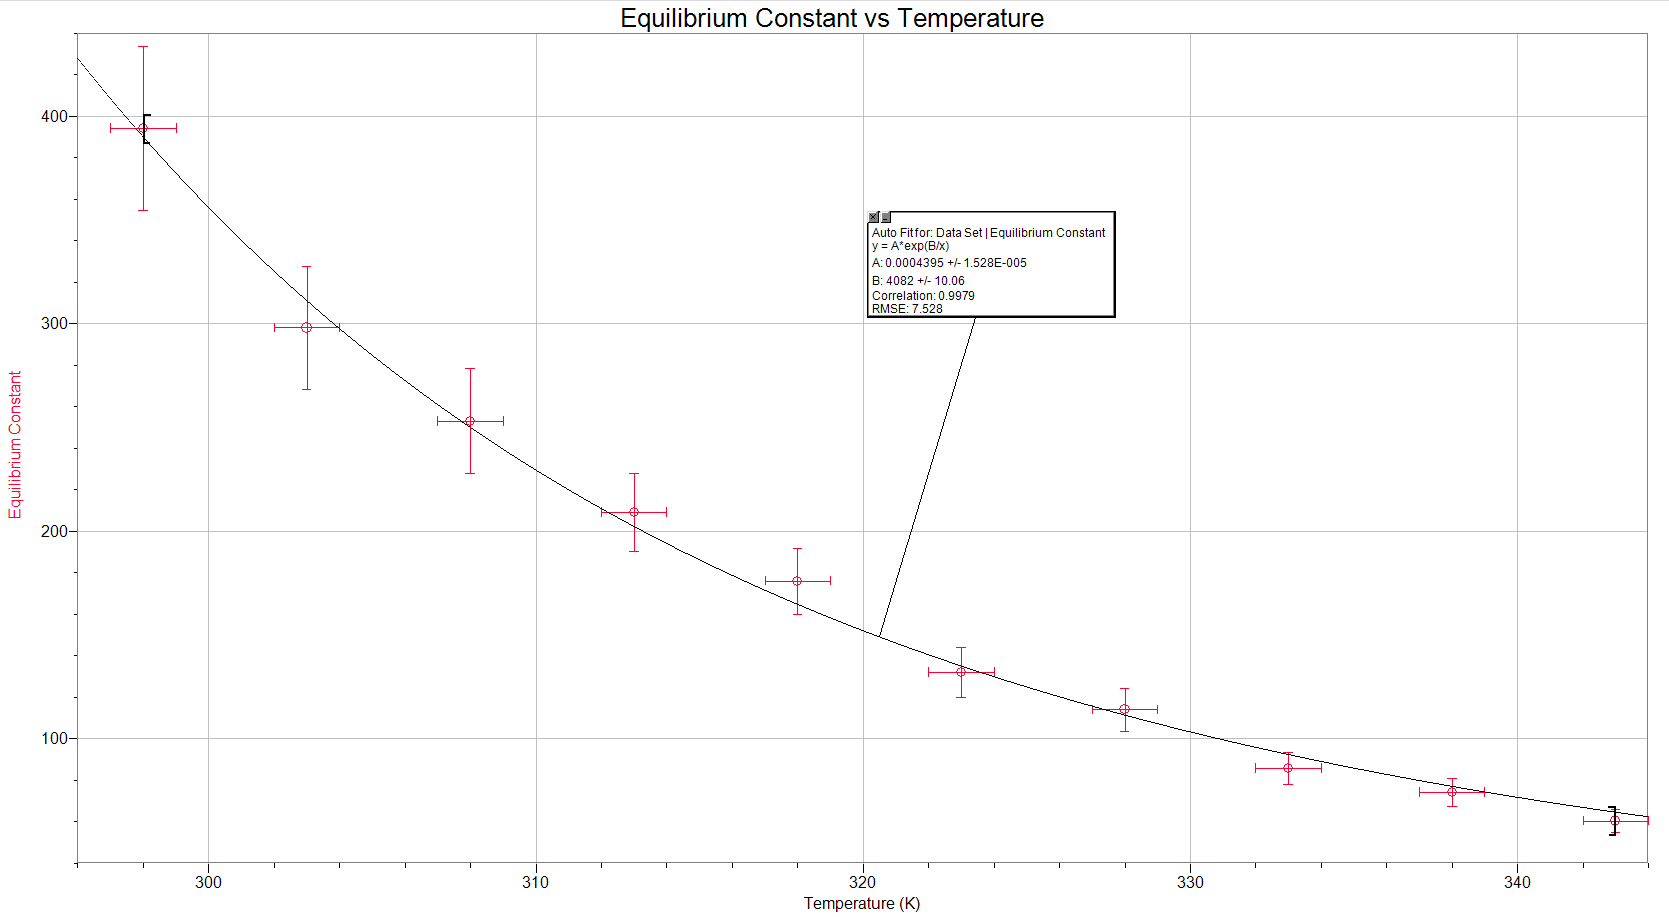
\includegraphics[width=100mm,height=\textheight,keepaspectratio]{images/before_linearization.png}
    \caption{Graph of Equilibrium Constant vs Temperature}
    \label{fig:before_linearization}
\end{figure}


\subsection{Linearization}
As seen in \cref{fig:before_linearization}, there is a very strong correlation (\(R^2=0.9979\)) to a \(K_c(T) = Ae^{B/T}\) curve, where A and B are coefficients. This matches the expected linearization as shown below.

\noindent
\newline
Setting the equations \(\Delta G^\circ = - RT\ln K_c\) and \(\Delta G^\circ = \Delta H^\circ - T \Delta S^\circ\) equal to each other.

\begin{align}
    - RT\ln K_c &= \Delta H^\circ - T \Delta S^\circ \\
    \ln K_c &= - \frac{\Delta H^\circ}{R} \times \frac{1}{T} + \frac{\Delta S^\circ}{R} \label{eq:linearization_theory}
\end{align}

\noindent
\cref{eq:linearization_theory} indicates that by taking the natural log of \(K_c\) and the reciprocal of temperature the relationship should be linear. A sample calculation is shown for this linearization.

\begin{equation}
    \textit{Reciprocal of Temperature} = \frac{1}{T_K} = \frac{1}{298 \; K} = 0.00336 K^{-1}
\end{equation}

\noindent
The uncertainty of \(\frac{1}{T_K}\) can be determined using \cref{eq:general_uncertainty}, 

\begin{align}
    \delta \left(\frac{1}{T_K}\right) &= \sqrt{\left(\frac{\partial \left(\frac{1}{T_K}\right)}{\partial T_K} \delta T_K \right)^2} = \frac{\delta T_K}{T^2} = \frac{1 \; K}{(298 \; K)^2} = 1 \times 10^{-5} \; K^{-1} \\
    \frac{\delta \left(\frac{1}{T_K}\right)}{\frac{1}{T_K}} &= 0.34\%
\end{align}

\noindent
Similarly,
\begin{equation}
    \textit{Natural Log of Equilibrium Constant} = \ln K_c = \ln 394 = 5.98
\end{equation}
\begin{align}
    \delta \ln K_c &= \sqrt{\left(\frac{\partial \ln K_c}{\partial T}\delta K_c \right)^2} = \frac{\delta K_c}{K_c} = \frac{37.59}{394} = 0.10 \\
    \frac{\delta \ln K_c}{\ln K_c} &= 1.8\%
\end{align}

\noindent
Repeating the above steps for each of the measurements to create \cref{table:after_linearization}.

\begin{table}[H]
\centering
\captionsetup{justification=centering,margin=2cm}
\resizebox{\textwidth}{!}{%
\begin{tabular}{|c|c|cccccccccccc|}
\hline
\multirow{2}{3cm}{\centering Reciprocal   of Temperature (1/K)} & \multirow{2}{4cm}{\centering Reciprocal of   Temperature Percent Uncertainty (\%)} & \multicolumn{12}{c|}{Natural Log of Equilibrium Constant}                                                                                                                                                                                                                                                                                                                                                                                                                                                                                \\ \cline{3-14} 
                                                   &                                                                       & \multicolumn{1}{c|}{Trial 1} & \multicolumn{1}{C{3cm}|}{Trial   1 Percent Uncertainty (\%)} & \multicolumn{1}{c|}{Trial   2} & \multicolumn{1}{C{3cm}|}{Trial   2 Percent Uncertainty (\%)} & \multicolumn{1}{c|}{Trial   3} & \multicolumn{1}{C{3cm}|}{Trial   3 Percent Uncertainty (\%)} & \multicolumn{1}{c|}{Trial   4} & \multicolumn{1}{C{3cm}|}{Trial   4 Percent Uncertainty (\%)} & \multicolumn{1}{c|}{Trial   5} & \multicolumn{1}{C{3cm}|}{Trial   5 Percent Uncertainty (\%)} & \multicolumn{1}{c|}{Trial   6} & \multicolumn{1}{C{3cm}|}{Trial   6 Percent Uncertainty (\%)} \\ \hline
0.00336                                            & 0.34                                                                  & \multicolumn{1}{c|}{5.98}    & \multicolumn{1}{c|}{1.8}                                & \multicolumn{1}{c|}{5.97}      & \multicolumn{1}{c|}{1.8}                                & \multicolumn{1}{c|}{5.92}      & \multicolumn{1}{c|}{1.7}                                & \multicolumn{1}{c|}{5.92}      & \multicolumn{1}{c|}{1.7}                                & \multicolumn{1}{c|}{6.00}      & \multicolumn{1}{c|}{1.8}                                & \multicolumn{1}{c|}{6.00}      & 1.8                                \\ \hline
0.00330                                            & 0.33                                                                  & \multicolumn{1}{c|}{5.70}    & \multicolumn{1}{c|}{1.7}                                & \multicolumn{1}{c|}{5.66}      & \multicolumn{1}{c|}{1.7}                                & \multicolumn{1}{c|}{5.68}      & \multicolumn{1}{c|}{1.7}                                & \multicolumn{1}{c|}{5.73}      & \multicolumn{1}{c|}{1.7}                                & \multicolumn{1}{c|}{5.67}      & \multicolumn{1}{c|}{1.7}                                & \multicolumn{1}{c|}{5.67}      & 1.7                                \\ \hline
0.00325                                            & 0.32                                                                  & \multicolumn{1}{c|}{5.53}    & \multicolumn{1}{c|}{1.7}                                & \multicolumn{1}{c|}{5.46}      & \multicolumn{1}{c|}{1.8}                                & \multicolumn{1}{c|}{5.47}      & \multicolumn{1}{c|}{1.8}                                & \multicolumn{1}{c|}{5.52}      & \multicolumn{1}{c|}{1.7}                                & \multicolumn{1}{c|}{5.46}      & \multicolumn{1}{c|}{1.8}                                & \multicolumn{1}{c|}{5.52}      & 1.7                                \\ \hline
0.00320                                            & 0.32                                                                  & \multicolumn{1}{c|}{5.34}    & \multicolumn{1}{c|}{1.8}                                & \multicolumn{1}{c|}{5.34}      & \multicolumn{1}{c|}{1.8}                                & \multicolumn{1}{c|}{5.32}      & \multicolumn{1}{c|}{1.8}                                & \multicolumn{1}{c|}{5.26}      & \multicolumn{1}{c|}{1.8}                                & \multicolumn{1}{c|}{5.25}      & \multicolumn{1}{c|}{1.8}                                & \multicolumn{1}{c|}{5.31}      & 1.8                                \\ \hline
0.00315                                            & 0.31                                                                  & \multicolumn{1}{c|}{5.17}    & \multicolumn{1}{c|}{1.8}                                & \multicolumn{1}{c|}{5.19}      & \multicolumn{1}{c|}{1.8}                                & \multicolumn{1}{c|}{5.19}      & \multicolumn{1}{c|}{1.8}                                & \multicolumn{1}{c|}{5.15}      & \multicolumn{1}{c|}{1.8}                                & \multicolumn{1}{c|}{5.14}      & \multicolumn{1}{c|}{1.8}                                & \multicolumn{1}{c|}{5.15}      & 1.8                                \\ \hline
0.00310                                            & 0.31                                                                  & \multicolumn{1}{c|}{4.88}    & \multicolumn{1}{c|}{1.9}                                & \multicolumn{1}{c|}{4.90}      & \multicolumn{1}{c|}{1.9}                                & \multicolumn{1}{c|}{4.98}      & \multicolumn{1}{c|}{1.8}                                & \multicolumn{1}{c|}{4.96}      & \multicolumn{1}{c|}{1.8}                                & \multicolumn{1}{c|}{4.92}      & \multicolumn{1}{c|}{1.9}                                & \multicolumn{1}{c|}{4.94}      & 1.9                                \\ \hline
0.00305                                            & 0.30                                                                  & \multicolumn{1}{c|}{4.73}    & \multicolumn{1}{c|}{1.9}                                & \multicolumn{1}{c|}{4.74}      & \multicolumn{1}{c|}{1.9}                                & \multicolumn{1}{c|}{4.76}      & \multicolumn{1}{c|}{1.9}                                & \multicolumn{1}{c|}{4.71}      & \multicolumn{1}{c|}{1.9}                                & \multicolumn{1}{c|}{4.73}      & \multicolumn{1}{c|}{1.9}                                & \multicolumn{1}{c|}{4.65}      & 2.0                                \\ \hline
0.00300                                            & 0.30                                                                  & \multicolumn{1}{c|}{4.45}    & \multicolumn{1}{c|}{2.0}                                & \multicolumn{1}{c|}{4.51}      & \multicolumn{1}{c|}{2.0}                                & \multicolumn{1}{c|}{4.54}      & \multicolumn{1}{c|}{2.0}                                & \multicolumn{1}{c|}{4.60}      & \multicolumn{1}{c|}{2.0}                                & \multicolumn{1}{c|}{4.62}      & \multicolumn{1}{c|}{2.0}                                & \multicolumn{1}{c|}{4.54}      & 2.0                                \\ \hline
0.00296                                            & 0.30                                                                  & \multicolumn{1}{c|}{4.31}    & \multicolumn{1}{c|}{2.0}                                & \multicolumn{1}{c|}{4.38}      & \multicolumn{1}{c|}{2.0}                                & \multicolumn{1}{c|}{4.47}      & \multicolumn{1}{c|}{2.0}                                & \multicolumn{1}{c|}{4.32}      & \multicolumn{1}{c|}{2.0}                                & \multicolumn{1}{c|}{4.43}      & \multicolumn{1}{c|}{2.0}                                & \multicolumn{1}{c|}{4.41}      & 2.0                                \\ \hline
0.00292                                            & 0.29                                                                  & \multicolumn{1}{c|}{4.10}    & \multicolumn{1}{c|}{2.0}                                & \multicolumn{1}{c|}{3.95}      & \multicolumn{1}{c|}{2.0}                                & \multicolumn{1}{c|}{4.02}      & \multicolumn{1}{c|}{2.0}                                & \multicolumn{1}{c|}{4.15}      & \multicolumn{1}{c|}{2.0}                                & \multicolumn{1}{c|}{4.13}      & \multicolumn{1}{c|}{2.0}                                & \multicolumn{1}{c|}{4.11}      & 2.0                                \\ \hline
\end{tabular}}
\end{table}

\begin{table}[H]
\centering
\captionsetup{justification=centering,margin=1cm}
\resizebox{\textwidth}{!}{%
\begin{tabular}{|cccccccccccccccc|}
\hline
\multicolumn{16}{|c|}{Natural Log of Equilibrium Constant (Continued.)}                                                                                                                                                                                                                                                                                                                                                                                                                                                                                                                                                            \\ \hline \multicolumn{1}{|c|}{Trial 7} & \multicolumn{1}{C{3cm}|}{Trial 7 Percent   Uncertainty (\%)} & \multicolumn{1}{|c|}{Trial 8} & \multicolumn{1}{C{3cm}|}{Trial 8 Percent   Uncertainty (\%)} & \multicolumn{1}{c|}{Trial 9} & \multicolumn{1}{C{3cm}|}{Trial 9 Percent   Uncertainty (\%)} & \multicolumn{1}{c|}{Trial 10} & \multicolumn{1}{C{3cm}|}{Trial 10   Percent Uncertainty (\%)} & \multicolumn{1}{c|}{Trial 11} & \multicolumn{1}{C{3cm}|}{Trial 11   Percent Uncertainty (\%)} & \multicolumn{1}{c|}{Trial 12} & \multicolumn{1}{C{3cm}|}{Trial 12   Percent Uncertainty (\%)} & \multicolumn{1}{c|}{Trial 13} & \multicolumn{1}{C{3cm}|}{Trial 13   Percent Uncertainty (\%)} & \multicolumn{1}{c|}{Trial 14} & \multicolumn{1}{C{3cm}|}{Trial 14   Percent Uncertainty (\%)} \\ \hline
\multicolumn{1}{|c|}{5.92}    & \multicolumn{1}{c|}{1.7}                                & \multicolumn{1}{c|}{5.98}    & \multicolumn{1}{c|}{1.8}                                & \multicolumn{1}{c|}{5.98}    & \multicolumn{1}{c|}{1.8}                                & \multicolumn{1}{c|}{5.97}     & \multicolumn{1}{c|}{1.8}                                 & \multicolumn{1}{c|}{5.97}     & \multicolumn{1}{c|}{1.8}                                 & \multicolumn{1}{c|}{6.01}     & \multicolumn{1}{c|}{1.8}                                 & \multicolumn{1}{c|}{5.99}     & \multicolumn{1}{c|}{1.8}                                 & \multicolumn{1}{c|}{5.95}     & 1.7                                 \\ \hline
\multicolumn{1}{|c|}{5.68}    & \multicolumn{1}{c|}{1.7}                                & \multicolumn{1}{c|}{5.66}    & \multicolumn{1}{c|}{1.7}                                & \multicolumn{1}{c|}{5.66}    & \multicolumn{1}{c|}{1.7}                                & \multicolumn{1}{c|}{5.69}     & \multicolumn{1}{c|}{1.7}                                 & \multicolumn{1}{c|}{5.73}     & \multicolumn{1}{c|}{1.7}                                 & \multicolumn{1}{c|}{5.67}     & \multicolumn{1}{c|}{1.7}                                 & \multicolumn{1}{c|}{5.70}     & \multicolumn{1}{c|}{1.7}                                 & \multicolumn{1}{c|}{5.68}     & 1.7                                 \\ \hline
\multicolumn{1}{|c|}{5.53}    & \multicolumn{1}{c|}{1.7}                                & \multicolumn{1}{c|}{5.47}    & \multicolumn{1}{c|}{1.8}                                & \multicolumn{1}{c|}{5.47}    & \multicolumn{1}{c|}{1.8}                                & \multicolumn{1}{c|}{5.53}     & \multicolumn{1}{c|}{1.7}                                 & \multicolumn{1}{c|}{5.46}     & \multicolumn{1}{c|}{1.8}                                 & \multicolumn{1}{c|}{5.47}     & \multicolumn{1}{c|}{1.8}                                 & \multicolumn{1}{c|}{5.53}     & \multicolumn{1}{c|}{1.7}                                 & \multicolumn{1}{c|}{5.52}     & 1.7                                 \\ \hline
\multicolumn{1}{|c|}{5.33}    & \multicolumn{1}{c|}{1.8}                                & \multicolumn{1}{c|}{5.36}    & \multicolumn{1}{c|}{1.8}                                & \multicolumn{1}{c|}{5.32}    & \multicolumn{1}{c|}{1.8}                                & \multicolumn{1}{c|}{5.26}     & \multicolumn{1}{c|}{1.8}                                 & \multicolumn{1}{c|}{5.32}     & \multicolumn{1}{c|}{1.8}                                 & \multicolumn{1}{c|}{5.32}     & \multicolumn{1}{c|}{1.8}                                 & \multicolumn{1}{c|}{5.35}     & \multicolumn{1}{c|}{1.8}                                 & \multicolumn{1}{c|}{5.37}     & 1.8                                 \\ \hline
\multicolumn{1}{|c|}{5.12}    & \multicolumn{1}{c|}{1.8}                                & \multicolumn{1}{c|}{5.17}    & \multicolumn{1}{c|}{1.8}                                & \multicolumn{1}{c|}{5.13}    & \multicolumn{1}{c|}{1.8}                                & \multicolumn{1}{c|}{5.12}     & \multicolumn{1}{c|}{1.8}                                 & \multicolumn{1}{c|}{5.13}     & \multicolumn{1}{c|}{1.8}                                 & \multicolumn{1}{c|}{5.16}     & \multicolumn{1}{c|}{1.8}                                 & \multicolumn{1}{c|}{5.12}     & \multicolumn{1}{c|}{1.8}                                 & \multicolumn{1}{c|}{5.13}     & 1.8                                 \\ \hline
\multicolumn{1}{|c|}{4.88}    & \multicolumn{1}{c|}{1.9}                                & \multicolumn{1}{c|}{4.92}    & \multicolumn{1}{c|}{1.9}                                & \multicolumn{1}{c|}{4.87}    & \multicolumn{1}{c|}{1.9}                                & \multicolumn{1}{c|}{4.89}     & \multicolumn{1}{c|}{1.9}                                 & \multicolumn{1}{c|}{4.89}     & \multicolumn{1}{c|}{1.9}                                 & \multicolumn{1}{c|}{4.88}     & \multicolumn{1}{c|}{1.9}                                 & \multicolumn{1}{c|}{4.87}     & \multicolumn{1}{c|}{1.9}                                 & \multicolumn{1}{c|}{4.89}     & 1.9                                 \\ \hline
\multicolumn{1}{|c|}{4.73}    & \multicolumn{1}{c|}{1.9}                                & \multicolumn{1}{c|}{4.74}    & \multicolumn{1}{c|}{1.9}                                & \multicolumn{1}{c|}{4.67}    & \multicolumn{1}{c|}{1.9}                                & \multicolumn{1}{c|}{4.69}     & \multicolumn{1}{c|}{1.9}                                 & \multicolumn{1}{c|}{4.64}     & \multicolumn{1}{c|}{2.0}                                 & \multicolumn{1}{c|}{4.74}     & \multicolumn{1}{c|}{1.9}                                 & \multicolumn{1}{c|}{4.75}     & \multicolumn{1}{c|}{1.9}                                 & \multicolumn{1}{c|}{4.69}     & 1.9                                 \\ \hline
\multicolumn{1}{|c|}{4.57}    & \multicolumn{1}{c|}{2.0}                                & \multicolumn{1}{c|}{4.55}    & \multicolumn{1}{c|}{2.0}                                & \multicolumn{1}{c|}{4.57}    & \multicolumn{1}{c|}{2.0}                                & \multicolumn{1}{c|}{4.57}     & \multicolumn{1}{c|}{2.0}                                 & \multicolumn{1}{c|}{4.56}     & \multicolumn{1}{c|}{2.0}                                 & \multicolumn{1}{c|}{4.64}     & \multicolumn{1}{c|}{2.0}                                 & \multicolumn{1}{c|}{4.61}     & \multicolumn{1}{c|}{2.0}                                 & \multicolumn{1}{c|}{4.60}     & 2.0                                 \\ \hline
\multicolumn{1}{|c|}{4.45}    & \multicolumn{1}{c|}{2.0}                                & \multicolumn{1}{c|}{4.35}    & \multicolumn{1}{c|}{2.0}                                & \multicolumn{1}{c|}{4.44}    & \multicolumn{1}{c|}{2.0}                                & \multicolumn{1}{c|}{4.33}     & \multicolumn{1}{c|}{2.0}                                 & \multicolumn{1}{c|}{4.31}     & \multicolumn{1}{c|}{2.0}                                 & \multicolumn{1}{c|}{4.45}     & \multicolumn{1}{c|}{2.0}                                 & \multicolumn{1}{c|}{4.43}     & \multicolumn{1}{c|}{2.0}                                 & \multicolumn{1}{c|}{4.42}     & 2.0                                 \\ \hline
\multicolumn{1}{|c|}{3.96}    & \multicolumn{1}{c|}{2.0}                                & \multicolumn{1}{c|}{3.97}    & \multicolumn{1}{c|}{2.0}                                & \multicolumn{1}{c|}{4.03}    & \multicolumn{1}{c|}{2.0}                                & \multicolumn{1}{c|}{3.93}     & \multicolumn{1}{c|}{2.0}                                 & \multicolumn{1}{c|}{4.04}     & \multicolumn{1}{c|}{2.0}                                 & \multicolumn{1}{c|}{4.15}     & \multicolumn{1}{c|}{2.0}                                 & \multicolumn{1}{c|}{4.11}     & \multicolumn{1}{c|}{2.0}                                 & \multicolumn{1}{c|}{4.01}     & 2.0                                 \\ \hline
\end{tabular}}
\caption{Natural Log of Equilibrium Constant vs Reciprocal of Temperature}
\label{table:after_linearization}
\end{table}

Finally, the average natural log of the equilibrium constant was determined for each of the reciprocal of temperature levels. The uncertainty of this average can be determined using the following formula. A sample calculation is shown below.

\begin{align}
    \delta (\ln K_c)_{avg} &= \frac{(\ln K_c)_{max} - (\ln K_c)_{min}}{2\sqrt{N}} = \frac{6.01 - 5.92}{2\sqrt{14}} = 0.01 \\
    \frac{\delta (\ln K_c)_{avg}}{(\ln K_c)_{avg}} &= 0.19\%
\end{align}

\noindent
Performing the average calculation for each reciprocal of temperature level, I created \cref{table:after_linearization_avg} and \cref{fig:after_linearization}.

\begin{table}[H]
\centering
\begin{tabular}{|c|c|c|c|}
\hline
\multicolumn{1}{|C{2.5cm}|}{Reciprocal   of Temperature (1/K)} & \multicolumn{1}{|C{4cm}|}{Reciprocal of   Temperature Percent Uncertainty (\%)} & \multicolumn{1}{|C{3.5cm}|}{Average Natural   Log of Equilibrium Constant} & \multicolumn{1}{|C{5cm}|}{Average Natural   Log of Equilibrium Constant Percent Uncertainty (\%)} \\ \hline
0.00336                           & 0.34                                                 & 5.97                                          & 0.19                                                                   \\ \hline
0.00330                           & 0.33                                                 & 5.68                                          & 0.18                                                                   \\ \hline
0.00325                           & 0.32                                                 & 5.50                                          & 0.19                                                                   \\ \hline
0.00320                           & 0.32                                                 & 5.32                                          & 0.31                                                                   \\ \hline
0.00315                           & 0.31                                                 & 5.15                                          & 0.17                                                                   \\ \hline
0.00310                           & 0.31                                                 & 4.90                                          & 0.30                                                                   \\ \hline
0.00305                           & 0.30                                                 & 4.71                                          & 0.36                                                                   \\ \hline
0.00300                           & 0.30                                                 & 4.57                                          & 0.55                                                                   \\ \hline
0.00296                           & 0.30                                                 & 4.39                                          & 0.49                                                                   \\ \hline
0.00292                           & 0.29                                                 & 4.05                                          & 0.73                                                                   \\ \hline
\end{tabular}
\caption{Average Natural Log of Equilibrium Constant vs Reciprocal of Temperature}
\label{table:after_linearization_avg}
\end{table}

\begin{figure}[H]
    \centering
    \captionsetup{justification=centering,margin=1.5cm}
    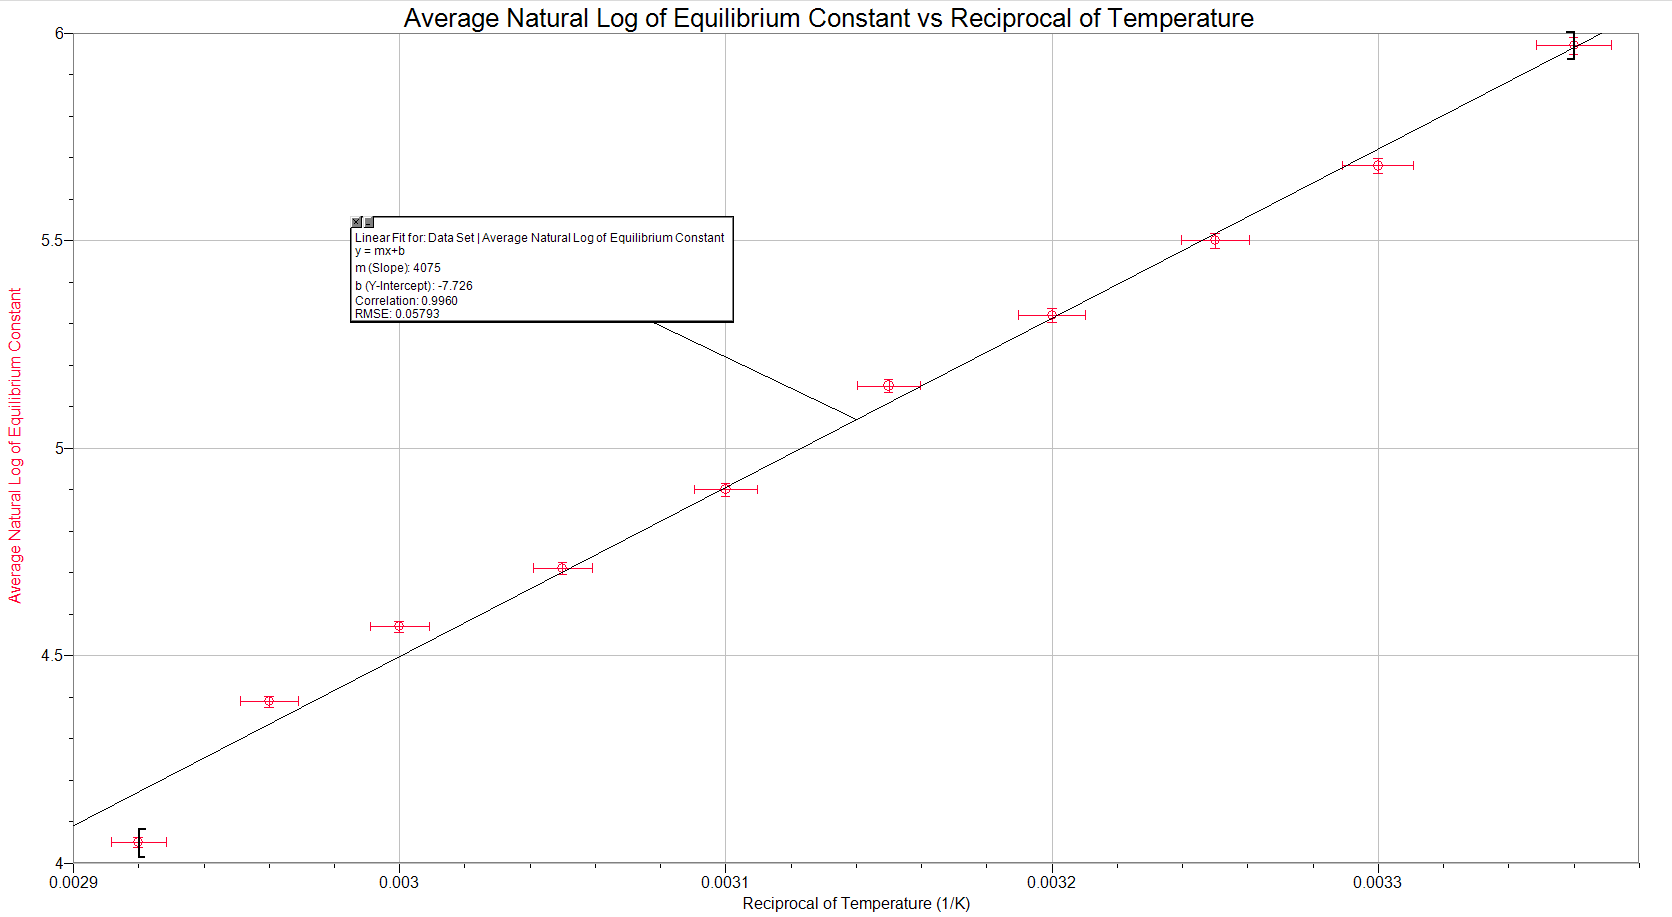
\includegraphics[width=100mm,height=\textheight,keepaspectratio]{images/after_linearization.png}
    \caption{Graph of Average Natural Log of Equilibrium Constant vs Reciprocal of Temperature}
    \label{fig:after_linearization}
\end{figure}

% \subsection{Percent Uncertainty and Percent Error of Slope}
% A rough estimate of the percent uncertainty of the slope $\beta$ can be determined by utilizing the maximum and minimum slope lines.
% \[\delta \beta = \frac{\beta_{max}-\beta_{min}}{2} = \frac{3719 K \ln{k\Omega}-3335 K \ln{k\Omega}}{2}=192 K \ln{k\Omega}\]
% \[\frac{\delta \beta}{\beta}=\frac{192 K \ln{k\Omega}}{3556 K \ln{k\Omega}}=5.40 \%\]

% The accepted value for the slope $\beta$ for this NTC Themistor is $3474 K \ln{k\Omega}$.
% Therefore, to calculate the percent error, the following calculation can be performed.
% \[Percent \; Error = \frac{|\beta_{actual} - \beta_{accepted}|}{\beta_{accepted}}=\frac{|3556 K \ln{k\Omega} - 3474 K \ln{k\Omega}|}{3474 K \ln{k\Omega}}=2.36\%\]


\subsection{Interpretation}
As seen in \cref{fig:after_linearization}), the line of best fit indicates a positive linear relationship between \(\ln K_c\) and \(\frac{1}{T}\). This means as \(\frac{1}{T}\) increases, \(\ln{K_c}\) will increase proportionally. Thus, this linearization proves that there is a negative exponential relationship between \(K_c\) and \(T\).

There is a very strong correlation (\(R^2=0.9960\)) between the linear regression and the linearized data. The line of best fit passes through almost all points and uncertainty bars. The minimum and maximum slope lines are very similar to the regression line. All this affirms that the \(K_c\) and \(T\) of a thiocynatoiron complex reaction follow a negative exponential relationship.

Finally, the slope and intercept of this linearized graph is proportional to the standard enthalpy change and entropy change of the reaction respectively, as shown in \cref{eq:linearization_theory}. Thus, the formation of the thiocynatoiron complex is exothermic and decreases entropy. The small \(\Delta H^\circ\) and \(\Delta S^\circ\) may be due to the formation of weak coordinate covalent bonds in the thiocyanatoiron complex.

\begin{align}
    \Delta H^\circ &= - m \times R = - 4075\; K \times 8.314 \; J \; mol^{-1} \; K^{-1} = -33880 \; J \; mol^{-1} \\
    \Delta S^\circ &= b \times R = -7.726 \times 8.314 \; J \; mol^{-1} \; K^{-1} = -64.23 \; J \; mol^{-1} \; K^{-1}
\end{align}